%%%%%%%%%%%%%%%%%%%%%%%%%%%%%%%%%%%%%%%%%%%%%%%%%%%%%%%%%%%%%%%%%%%%%%%%%%%%%%%%
%2345678901234567890123456789012345678901234567890123456789012345678901234567890
%        1         2         3         4         5         6         7         8

\documentclass[letterpaper, 10 pt, conference]{ieeeconf}  % Comment this line out if you need a4paper

% \documentclass[letterpaper, 12 pt, twoside]{report}  % Comment this line out if you need a4paper


%\documentclass[a4paper, 10pt, conference]{ieeeconf} % Use this line for a4 paper able to be

% \IEEEoverridecommandlockouts %This command is only needed if you want to use the \thanks command

\overrideIEEEmargins  % Needed to meet printer requirements.

%In case you encounter the following error:
%Error 1010 The PDF file may be corrupt (unable to open PDF file) OR
%Error 1000 An error occurred while parsing a contents stream. Unable to analyze the PDF file.
%This is a known problem with pdfLaTeX conversion filter. The file cannot be opened with acrobat reader
%Please use one of the alternatives below to circumvent this error by uncommenting one or the other
%\pdfobjcompresslevel=0
%\pdfminorversion=4

% See the \addtolength command later in the file to balance the column lengths
% on the last page of the document

% The following packages can be found on http:\\www.ctan.org
\usepackage{graphicx} % for pdf, bitmapped graphics files
%\usepackage{epsfig} % for postscript graphics files
%\usepackage{mathptmx} % assumes new font selection scheme installed
%\usepackage{times} % assumes new font selection scheme installed
\usepackage{amsmath} % assumes amsmath package installed
\usepackage{amssymb}  % assumes amsmath package installed
%\usepackage{dsfont}
\usepackage{algorithm}
\usepackage{algorithmic}
\usepackage{commath}

\usepackage{xcolor}
\newcommand{\todo}[1]{{\color{blue}[TODO: #1]}}
\newcommand{\comment}[1]{{\color{red}[COMMENT: #1]}}
\newcommand{\response}[1]{{\color{green}[RESPONSE: #1]}}
\graphicspath{{figures/}}


\DeclareMathOperator*{\argmax}{arg\,max}
\DeclareMathOperator*{\argmin}{arg\,min}

\title{\LARGE \bf
Multi-Agent Autonomous Mapping of Unknown GPS-Denied Environments Using a Relative Navigation Framework}

\author{Jacob M. Olson$^{1}$, Timothy W. McLain$^{2}$% <-this % stops a space
\thanks{Thanks to Mathieu Labbe for being responsive to answering questions on the RTAB-Map forum and helping with developing the map merging node.}% <-this % stops a space
\thanks{$^{1}$The corresponding author can be contacted at
        {\tt\small jacobmo at byu.edu}.}%
\thanks{$^{2}$All authors are with the Department of Mechanical Engineering or Electrical and Computer Engineering,
        Brigham Young University, Provo, UT, 84602, USA.}%
%\thanks{$^{3}$C. Peterson is with the Faculty of Electrical and Computer Engineering,
%		Brigham Young University, Provo, UT, 84602, USA.
%        {\tt\small cammy.peterson at byu.edu}}%
%\thanks{$^{4}$R. W. Beard is with the Faculty of Electrical and Computer Engineering,
%		Brigham Young University, Provo, UT, 84602, USA.
%        {\tt\small beard at byu.edu}}%
}

\begin{document}

\maketitle
\thispagestyle{empty}
\pagestyle{empty}


%%%%%%%%%%%%%%%%%%%%%%%%%%%%%%%%%%%%%%%%%%%%%%%%%%%%%%%%%%%%%%%%%%%%%%%%%%%%%%%%
\begin{abstract}

When generating 3D maps with unmanned aerial vehicles (UAVs) in GPS-denied environments, it is important to correctly handle path planning, estimation, and mapping techniques. Because multirotor UAVs are limited in flight time, using multiple UAVs to map an environment collaboratively can significantly improve the mapping efficiency. To solve this problem, we propose the following strategies: Use a combination of a reactive path planner with an obstacle avoidance velocity filter to handle navigation in complex environments. Estimate the relative and global states of UAVs separately with a relative navigation framework to allow for loop closures in the mapping process without causing the estimation to diverge. Use a graph based simultaneous localization and mapping (graph-SLAM) technique on multiple UAVs simultaneously and merge the maps of the UAVs in real-time. These methods allow for efficient autonomous mapping of complex GPS-denied environments. 

\end{abstract}


%%%%%%%%%%%%%%%%%%%%%%%%%%%%%%%%%%%%%%%%%%%%%%%%%%%%%%%%%%%%%%%%%%%%%%%%%%%%%%%%
\section{Introduction}

\comment{Add more motivation here? like search and rescue, need for dense maps?}
Mapping and navigating an environment where GPS (global positioning system) signals are degraded or entirely unavailable such as an earthquake damaged building is not a trivial task. Often these GPS-denied environments are inaccessible to ground robots due to difficult terrain. This lends itself better to the use use of UAVs (unmanned aerial vehicles) to carry out some or all of the mapping. When navigating indoor environments with a UAV, collision with any obstacles can be catastrophic. Measures must be taken to avoid any collisions. We use a combination of a high-level reactive path planner and a low-level obstacle avoidance filter to avoid obstacles.

To be successful, most dense mapping approaches rely on high quality GPS measurements to patch together data to generate a map \cite{Siebert2014, Martin2015}. These methods break down when GPS is not available because the global position must be estimated rather than measured. To overcome the lack of GPS some form of simultaneous localization and mapping (SLAM) with visual odometry must be used. We use a form of graph-SLAM with a 3D camera and depth-enhanced visual odometry.

Because of the limited flight time of UAVs, mapping large areas with a single UAV can be inefficient. The mapping process can be streamlined by dividing the area between multiple UAVs. Each mapping a portion of the environment then combining all of the maps into a single one. One recent approach to this problem by Micheal et al. was to use a ground robot and a UAV to collaboratively map an earthquake damaged building. In this research, the UAV acted as an extension to the ground robot, flying into the difficult terrain to build onto the map started by the ground robot \cite{Michael2012}. More recently, Mangelson et al. detailed a method to effectively merge maps collected from multiple robots acting separately \cite{Mangelson2018}. In our approach, we use multiple UAVs flying simultaneously to map an indoor GPS-denied environment. The method we propose also combines the maps from the UAVs into a single map in near real time.

The remainder of the paper is organized as follows: Section \ref{approach} describes the framework used to navigate and map the environment, and background on what previous work has made this research possible. Section \ref{planning} details the planning and control schemes used to successfully navigate the unknown area. The method used to combine maps in near real-time is then explained in Section \ref{merge}. Results showing and evaluating the generated maps are presented in Section \ref{results}. Finally, conclusions are presented in Section \ref{conclusions}.

%%%%%%%%%%%%%%%%%%%%%%%%%%%%%%%%%%%%%%%%%%%%%%%%%%%%%%%%%%%%%%%%%%%%%%%%%%%%%%%%
\section{Technical Approach}\label{approach}

\subsection{Problem Statement}

The goal of this paper is to show how to successfully navigate and map a GPS-denied environment using multiple UAVs collaborating with each other. For map building to be successful, flight paths that produce high quality loop closures and good coverage of the environment are required. The framework presented in this section assumes that high quality paths will be supplied either by the user or by a high-level coverage path planner. Rather than focus on path generation, the focus of this paper is first, to show that properly estimating UAV states allows for successful GPS-denied navigation, and second, to demonstrate how to streamline the mapping process by merging multiple maps into a single map. A high-level network diagram is shown in Fig. \ref{fig:rtab_network} which outlines the framework used in this paper to successfully generate a single merged map from multiple UAVs in a GPS denied environment. Each section of the diagram will be described in detail throughout the paper.

\begin{figure*}
\centering
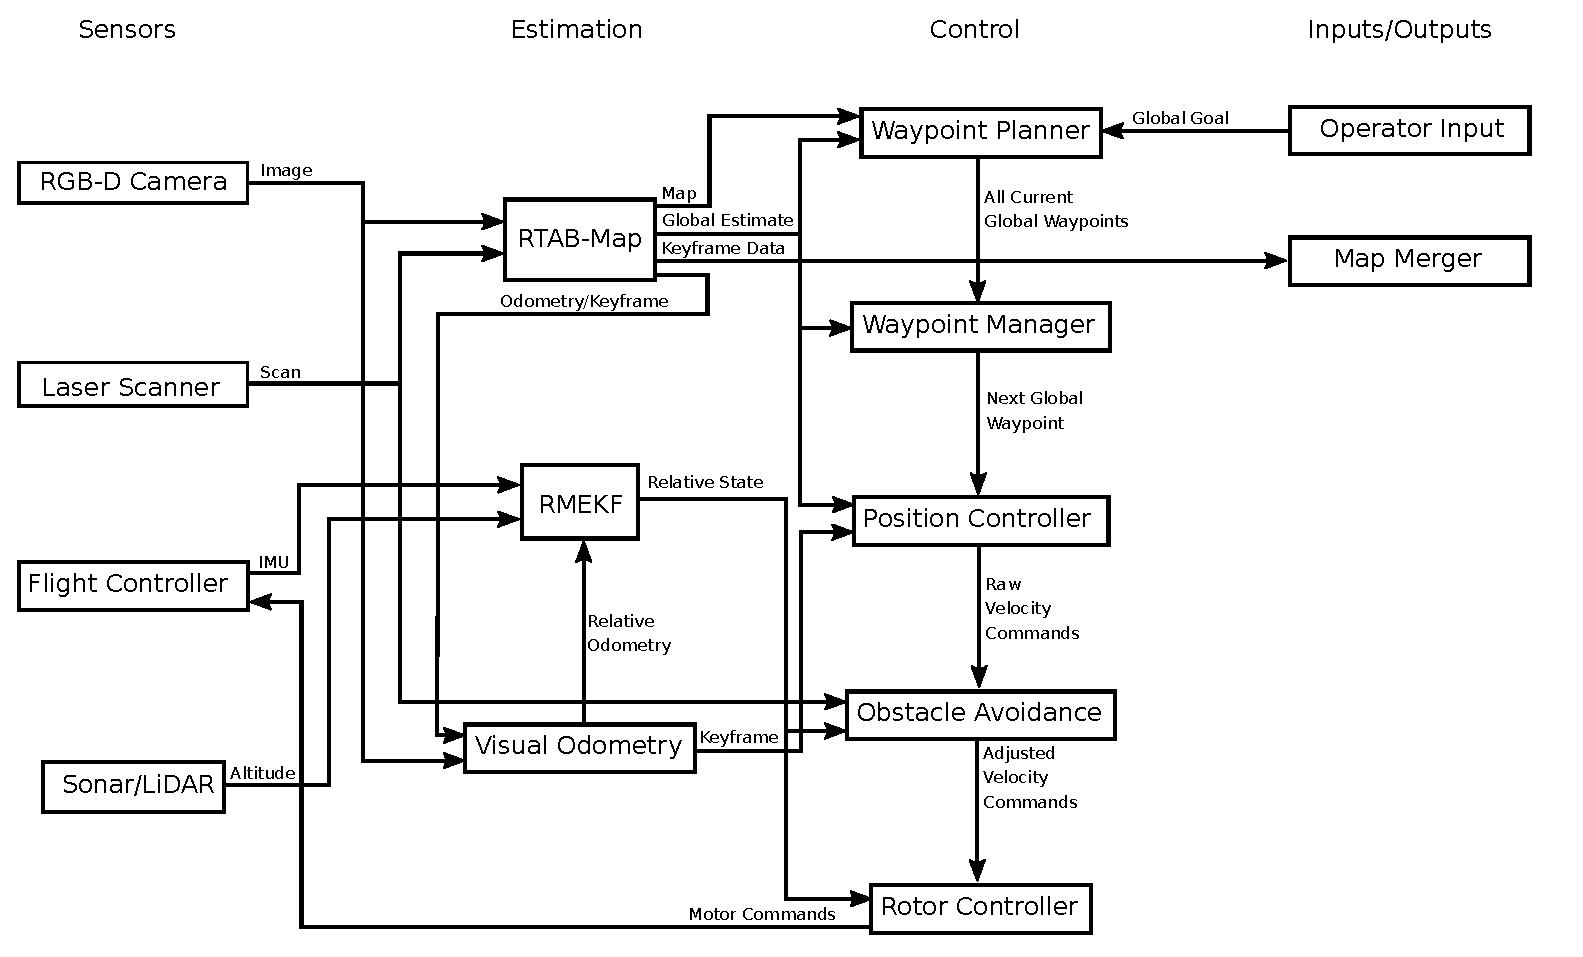
\includegraphics[width=1.0\linewidth]{rtab_relative_nav_network}
\caption{The network diagram of the relative navigation framework proposed in this paper}
\label{fig:rtab_network}
\end{figure*}

\subsection{Sensors}

Since we are operating in a GPS-denied environment, we are not able to rely on GPS measurements to give us global information about where the UAVs are located. The sensors used by the UAV to estimate its state are a 3D color and depth (RGB-D) camera (Intel RealSense D435 \cite{Intel}), a planar light detection and ranging (LiDAR) laser scanner, a single-beam LiDAR range finder, and an inertial measurement unit (IMU) on the onboard flight controller. Using only these sensors and the flight computer, we accurately estimate the states of the UAV enough control its attitude and position. The following section elaborates on how these sensors are used in the estimation.

\subsection{Estimation}

Estimation is the most critical element in enabling autonomous flight. Without good position and attitude estimation, autonomous navigation algorithms cease to function. We use a graph-SLAM approach similar to that developed by Thrun et al. \cite{Thrun2006} to navigate and generate the maps. Loop closures, which occur when a robot sees the same objects from similar locations at different points in time, can cause estimators to diverge if they are not handled correctly. Every time a new loop closure occurs, the map and position estimate are re-optimized. If the new loop closure results in a large shift in the current position estimate, a naive estimator can diverge because of the discontinuity of the estimated global position. To avoid the issue of loop closures causing instability in the controller, we estimate the global and relative states of the UAV separately and do not rely on the global state estimate to control the attitude of the UAV.

We store the current global state estimates in a transformation tree as shown in Fig. \ref{fig:tf_tree}. The $\mathit{world}$ frame is the inertial NED (north east down) frame of the world. It is fixed and does not change over time. The UAV's starting location with respect to the world is set as the $\mathit{map}$ frame which is represented in the inertial NWU (north west up) orientation. The $\mathit{base\_link}$ frame represents the current estimated position of the the UAV in the NED orientation with the $\mathit{camera\_link}$ frame representing the position in the NWU orientation. The $\mathit{camera\_base\_link}$ frame represents the current position of the camera in the camera frame.

The $\mathit{odom}$ frame is used to adjust for loop closures. When the flight begins, the $\mathit{odom}$ frame starts with zero offset from the $\mathit{map}$ frame. Every time a loop closure is detected and the map is re-optimized, the transform between the $\mathit{map}$ and $\mathit{odom}$ frames is adjusted to reflect the correction. This allows the transform between the $\mathit{odom}$ frame and the robot frames ($\mathit{camera\_link}$ and $\mathit{base\_link}$) to stay continuous when loop closures are detected even though the position estimate demonstrates not.

The $\mathit{keyframe}$, $\mathit{keyframe\_world}$ and $\mathit{keyframe\_camera}$ frames are used to track the relative visual odometry used by the relative estimator. More specifically, the relative visual odometry is stored in the tree as the transform between the $\mathit{keyframe}$ and $\mathit{camera\_link}$ frames in the NWU orientation. For convenience, we also keep track of the the NWU orientation with the $\mathit{keyframe\_world}$ frame and the camera orientation with the $\mathit{keyframe\_camera}$ frame.

The UAV's current waypoint is represented as the transform between the $\mathit{world}$ and $\mathit{waypoint}$ frames. This way a loop closure does not shift the desired global position of the waypoint. The position controller operates on the error between the $\mathit{waypoint}$ and $\mathit{base\_link}$ frames.

More detail regarding the uses and implementations of these transforms will be further explained in the following sections.

%This is under the assumption that the desired waypoint location is known globaly, this could be modified to set the new waypoint relative to odom frame if the position is relative to the current obstacles rather than the global position.

\begin{figure*}
\centering
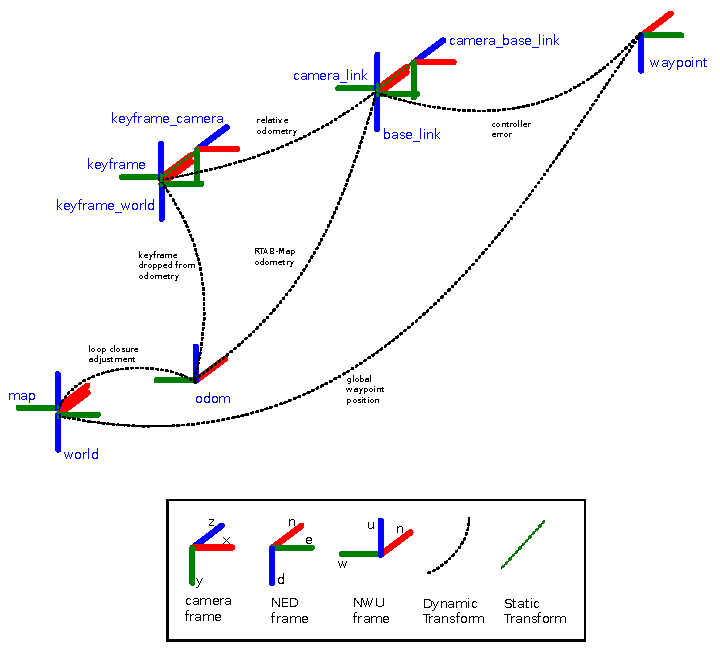
\includegraphics[width=0.9\linewidth]{tf_tree_relative_rtab}
\caption{The transformation tree of the reference frames used in estimation and control.}
\label{fig:tf_tree}
\end{figure*}

\subsubsection{RTAB-Map}

RTAB-Map (real-time appearence-based mapping), developed by Labbe et al. \cite{Labbe2011}\cite{Labbe2013}\cite{Labbe2019}, is a powerful open source software library that uses graph-SLAM with appearance-based loop closures to generate high-quality, dense 3D maps using only a RGB-D camera and a planar laser scanner. When coupled with its depth enhanced visual odometry algorithm called RGBD-Odometry \cite{Labbe2019}, it is able to accurately estimate the UAVs position with respect to the map that is being built. Unlike the odometry, the map building uses a keframe based approach. Rather that try to use each camera frame to build the map and optimize the graph, it periodically saves off the camera frame information at a set rate (we used 1 Hz) and declares a new keyframe.  Then only these keyframes are used to build the map and optimize the graph. RTAB-Map is primarily designed for use with slow moving ground robots which do not need high-rate state estimation to work. Since RTAB-Map does not use an IMU or altimiter, the highest rate of estimation is the visual odometry which is limited by the frame rate of the camera. We found the estimation rate of RTAB-Map on our hardware to be in the 10-30 Hz range which is not sufficient on its own to use for autonomous navigation with a UAV. We used the state estimates from the RGBD-Odometry node as an input to the estimation for the relative framework.

Although the current functionality of RTAB-Map does allow for multi-session mapping, it does not allow for multiple agents mapping simultaneously to combine the maps into a single one. This paper proposes a method to extend the functionality of RTAB-Map to combine the maps of multiple agents flying simultaneously into a single map in near real time. The implementation of this method is detailed in section \ref{merge}.

RTAB-Map manages the $\mathit{map}$, $\mathit{odom}$, $\mathit{base\_link}$, $\mathit{camera\_link}$, and $\mathit{camera\_base\_link}$ frames in the transformation tree as previously described. Along with the frames, it handles all of the loop closures and graph optimization.

We use the current position estimate produced by RTAB-Map for the position controller and waypoint manager. Because of the inevitable inaccuracies and the lower estimate rates of RTAB-Map, we do not use these estimates to perform attitude control on the UAVs. Rather, we use a relative navigation framework to estimate the attitude and relative state.

\subsubsection{Visual Odometry} \label{vis_odom}

The odometry and keyframe information generated by RTAB-Map is used to produce a relative odometry message that is sent the relative estimator. RTAB-Map produces a global visual odometry which provides a real time estimate of the global position and orientation of the UAV. Each time a new keyframe is declared, a new node is added to the graph, and the visual odometry node shown in Fig \ref{fig:rtab_network} resets the transform between the $\mathit{keyframe}$ and $\mathit{camera\_link}$ frames to zero. As previously mentioned, this relative odometry information is stored as the transform between the $\mathit{keyframe}$ and $\mathit{camera\_link}$ frames. The relative odometry only tracks the UAVs movement with respect to the last keyframe that was declared. Because of the constant resetting of the keyframe transform, the odometry used by the relative estimator is less susceptible to drift over time.

\subsubsection{RMEKF}

The relative navigation framework established by Wheeler et al. \cite{Wheeler2017}\cite{Wheeler2018} and Koch et al. \cite{Koch2017} has been shown to successfully estimate the UAV's relative state sufficient to autonomously navigate in GPS-denied environments that had been previously mapped. Thus far, however, it has not been extended to estimation and navigation in unknown and unmapped environments, this paper proposes a method to extend the functionality to these environments.

The Relative Multiplicative Extended Kalman Filter (RMEKF) is the heart of the relative framework. It uses the IMU measurement from the flight controller, the relative visual odometry as explained previously, and the attitude measurement from the LiDAR single beam range finder as the measurement updates. Then using the multirotor dynamics model, the RMEKF is able to accurately estimate the relative state of the UAV with respect to the previous keyframe. This estimate is used for obstacle avoidance and high-rate attitude control. The RMEKF makes no effort to estimate the global position of the UAV. As a result, corrections in the estimated global position from loop closures and drift in visual odometry do not cause the estimator to diverge, thus avoiding stability issues in the velocity and attitude controllers onboard the UAV.

\subsection{Control}

To successfully control a UAV using the relative navigation framework, the control must be segmented into different tiers to take advantage of both global and relative estimates.

\subsubsection{Waypoint Planner}

The first stage of the cascading control is the waypoint planner. The inputs to the planner are the global goal, the current known obstacles, and the current global estimates. It outputs a path to the goal that avoids all known obstacles as set of waypoints. This stage will be further explained in Section \ref{planning}.

\subsubsection{Waypoint Manager}

After receiving the current set of waypoints, the waypoint manager selects the appropriate current waypoint for the UAV and sends the global location to the position controller. The waypoint manager monitors the position and heading error between the current estimated position and the current waypoint. When the error crosses below a user-defined threshold value, the next waypoint is sent to the position controller.

\subsubsection{Position Controller}

The position controller drives the error between the current estimated position and heading of the UAV and the next waypoint to zero. Since it operates in the error space of the the UAV rather than the state space, sudden shifts in the UAVs position estimate caused by loop closures have minimal effect on the controller and it is able to continue controlling the error to zero. The output of the position controller is a velocity command.

\subsubsection{Obstacle Avoidance} \label{obs_avoid}

Before passing the velocity control into the attitude controller, it is filtered through an obstacle avoidance algorithm. This algorithm uses the current relative estimates from the RMEKF and current obstacles detected by the planar laser scanner to modify the input velocity command. It uses a cushioned extended-periphery avoidance (CEPA) technique developed by Jackson et al. \cite{Jackson2016} to alter the velocity command when necessary by pushing the UAV away from obstacles while changing the incoming velocity command as little as possible. The obstacle avoidance node then sends the modified velocity command to the attitude controller.

\subsubsection{Attitude Controller}

The attitude controller is a conventional PID controller that takes the velocity input commands and outputs the motor commands to the flight controller.

\subsection{Inputs/Outputs}

The input for each agent in the system is the desired goal location either from operator input or from a high level path planner. As each agent maps the environment, keyframe data consisting of the color and depth images and feature descriptions from the images is sent to the map merger each time a new keyframe is declared. The map merger will be further explored in Section \ref{merge}.

%%%%%%%%%%%%%%%%%%%%%%%%%%%%%%%%%%%%%%%%%%%%%%%%%%%%%%%%%%%%%%%%%%%%%%%%%%%%%%%%
\section{Planning}\label{planning}

\comment{too much background? or not enough explanation?} When designing the reactive planner, we explored using both node based optimal algorithms and sampling based algorithms \cite{Yang2016}. Node based, or heuristic search algorithms like A* work well to find feasible paths around obstacles are able to guarantee optimality \cite{Nilsson2011}. The downside to these is that in order to plan, they need to exhaustively search the design area. This makes them less efficient to use when the map is large and constantly changing. They also require the planning area to be discretized which can result in the planner not finding paths to the goal in a complex map if the area is discretized too much. Sampling based algorithms, like rapidly-exploring random trees (RRT) which was originally developed by Lavalle et al. \cite{Lavalle1998} are effective for planning in real time with dynamic obstacles. They randomly search the full, non-discretized map for feasible paths rather than requiring an exhaustive search. Statistically, RRT planning is much less computationally intensive each time a new path is planned, than A*. RRT planning does not guarantee optimal paths, but if a path to the goal exists it will find a path and usually with less computation than A*. More recently, improvements to RRT have been explored such as RRT* developed by Karaman et al. \cite{Karaman2011} which is able to guarantee asymptotically optimal paths by modifying the search tree. Since our planner is used as a form of exploration of unknown environments, we decided to not extend the planner to use RRT* to allow it to be more random in the flight path to encourage more exploration of the map while flying paths.

We used a form of RRT with a path smoothing approach similar to that proposed by Beard and McLain in 2012 \cite{Beard2012} to improve and simplify the resultant paths. Since our planner uses a dense 2D grid map of all currently known obstacles, some adjustments are needed for it to efficiently plan and re-plan when new obstacles are discovered in the current path.

\subsection{Global Goal Following with Relative Estimation}

As mentioned earlier, the relative estimator critical to keeping the UAV airborne only estimates its relative state with respect to the last keyframe and makes no attempt to estimate the global position of the UAV. By doing so, the global estimate of the position does not have to be continuous and is able to slide and adjust with loop closure corrections without affecting the estimator. The path planner generates a global path from the current position to the goal. The global paths do not adjust with loop closures and the map is continually changing as the UAV flies. For either of these reasons, obstacles can appear in the path at any time. To avoid these obstacles, the planner dynamically re-plans paths any time an obstacle is detected in the path.

\subsection{Reactive Path Planning}

Fig. \ref{fig:reactive_plan} shows the process of how the dynamic path planner would work in an example scenario. When the UAV starts, little is known about the environment. The only obstacles in the map are the ones that are within line-of-sight of the laser scanner when the flight begins. A path is planned to the goal which avoids the obstacles that are initially detected. As the UAV flies, the obstacle map is continuously updated with new obstacles and the path is constantly being checked for collisions. If collisions are found, a new path is planned to the goal from the current location which avoids the newly discovered obstacles. This process continues until the agent is able to successfully reach the goal. Since the path is updated any time a potential collision is detected, no prior knowledge of the environment is required to begin flying.

\begin{figure*}
\centering
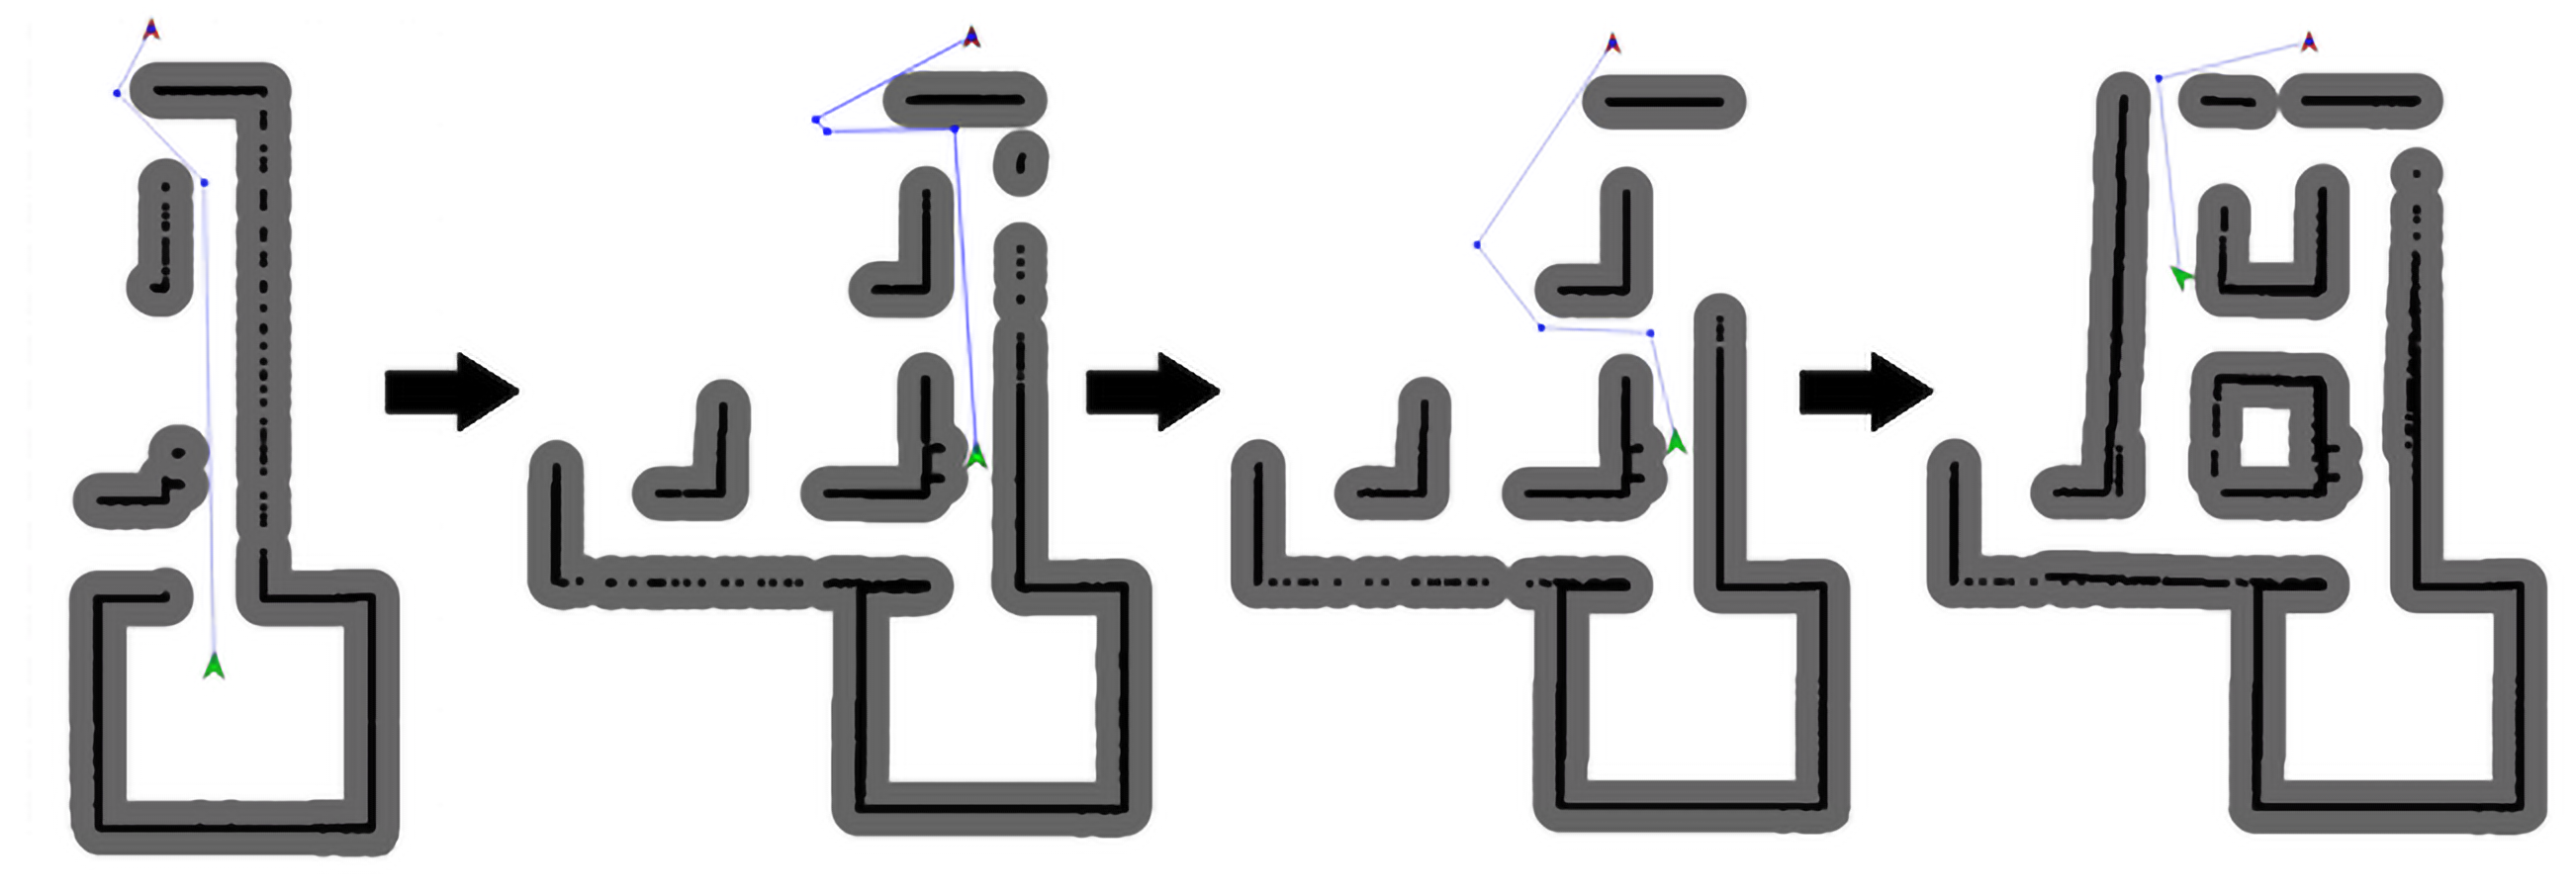
\includegraphics[width=1.0\linewidth]{adaptive_path_plan2.png}
\caption{An example of how the reactive path planner works as the UAV flies the planned path. The current estimated position is marked by the green arrow, the current goal position is marked by the red arrow, and the current path is marked with blue lines. Detected obstacles and safety buffers are represented with black and grey respectively.}
\label{fig:reactive_plan}
\end{figure*}

The planner also includes a buffer around each detected obstacle to avoid planning paths that would cause the UAV to fly too close to obstacles. The buffer size is set by the user, but is always at least half the width of the UAV. This ensures that any waypoint is far enough away from obstacles that it can be reached without any part of the UAV touching an obstacle.

Since this planner is used in conjunction with the CEPA obstacle avoidance node explained in \ref{obs_avoid}, the UAV is able to effectively avoid obstacles in emergency situations by correcting any velocity command that would have caused a collision. The UAV is also able to navigate through complex maps that would not be possible with only obstacle avoidance.

\subsubsection{Efficient Collision Detection}
Most implementations of RRT only deal with a small number of obstacles. The obstacles we use are from a 2D grid map generated by RTAB-Map so rather than having just a few large obstacles, there are many small obstacles. Using a standard obstacle detection check with each propagation of the RRT would be extremely inefficient. To maximize the efficiency during planning, we use a strategy that allows the planner to ignore most obstacles in the map when performing collision checks. An example of how this works is illustrated in Fig. \ref{fig:rrt_sample}.

\begin{figure}
\centering
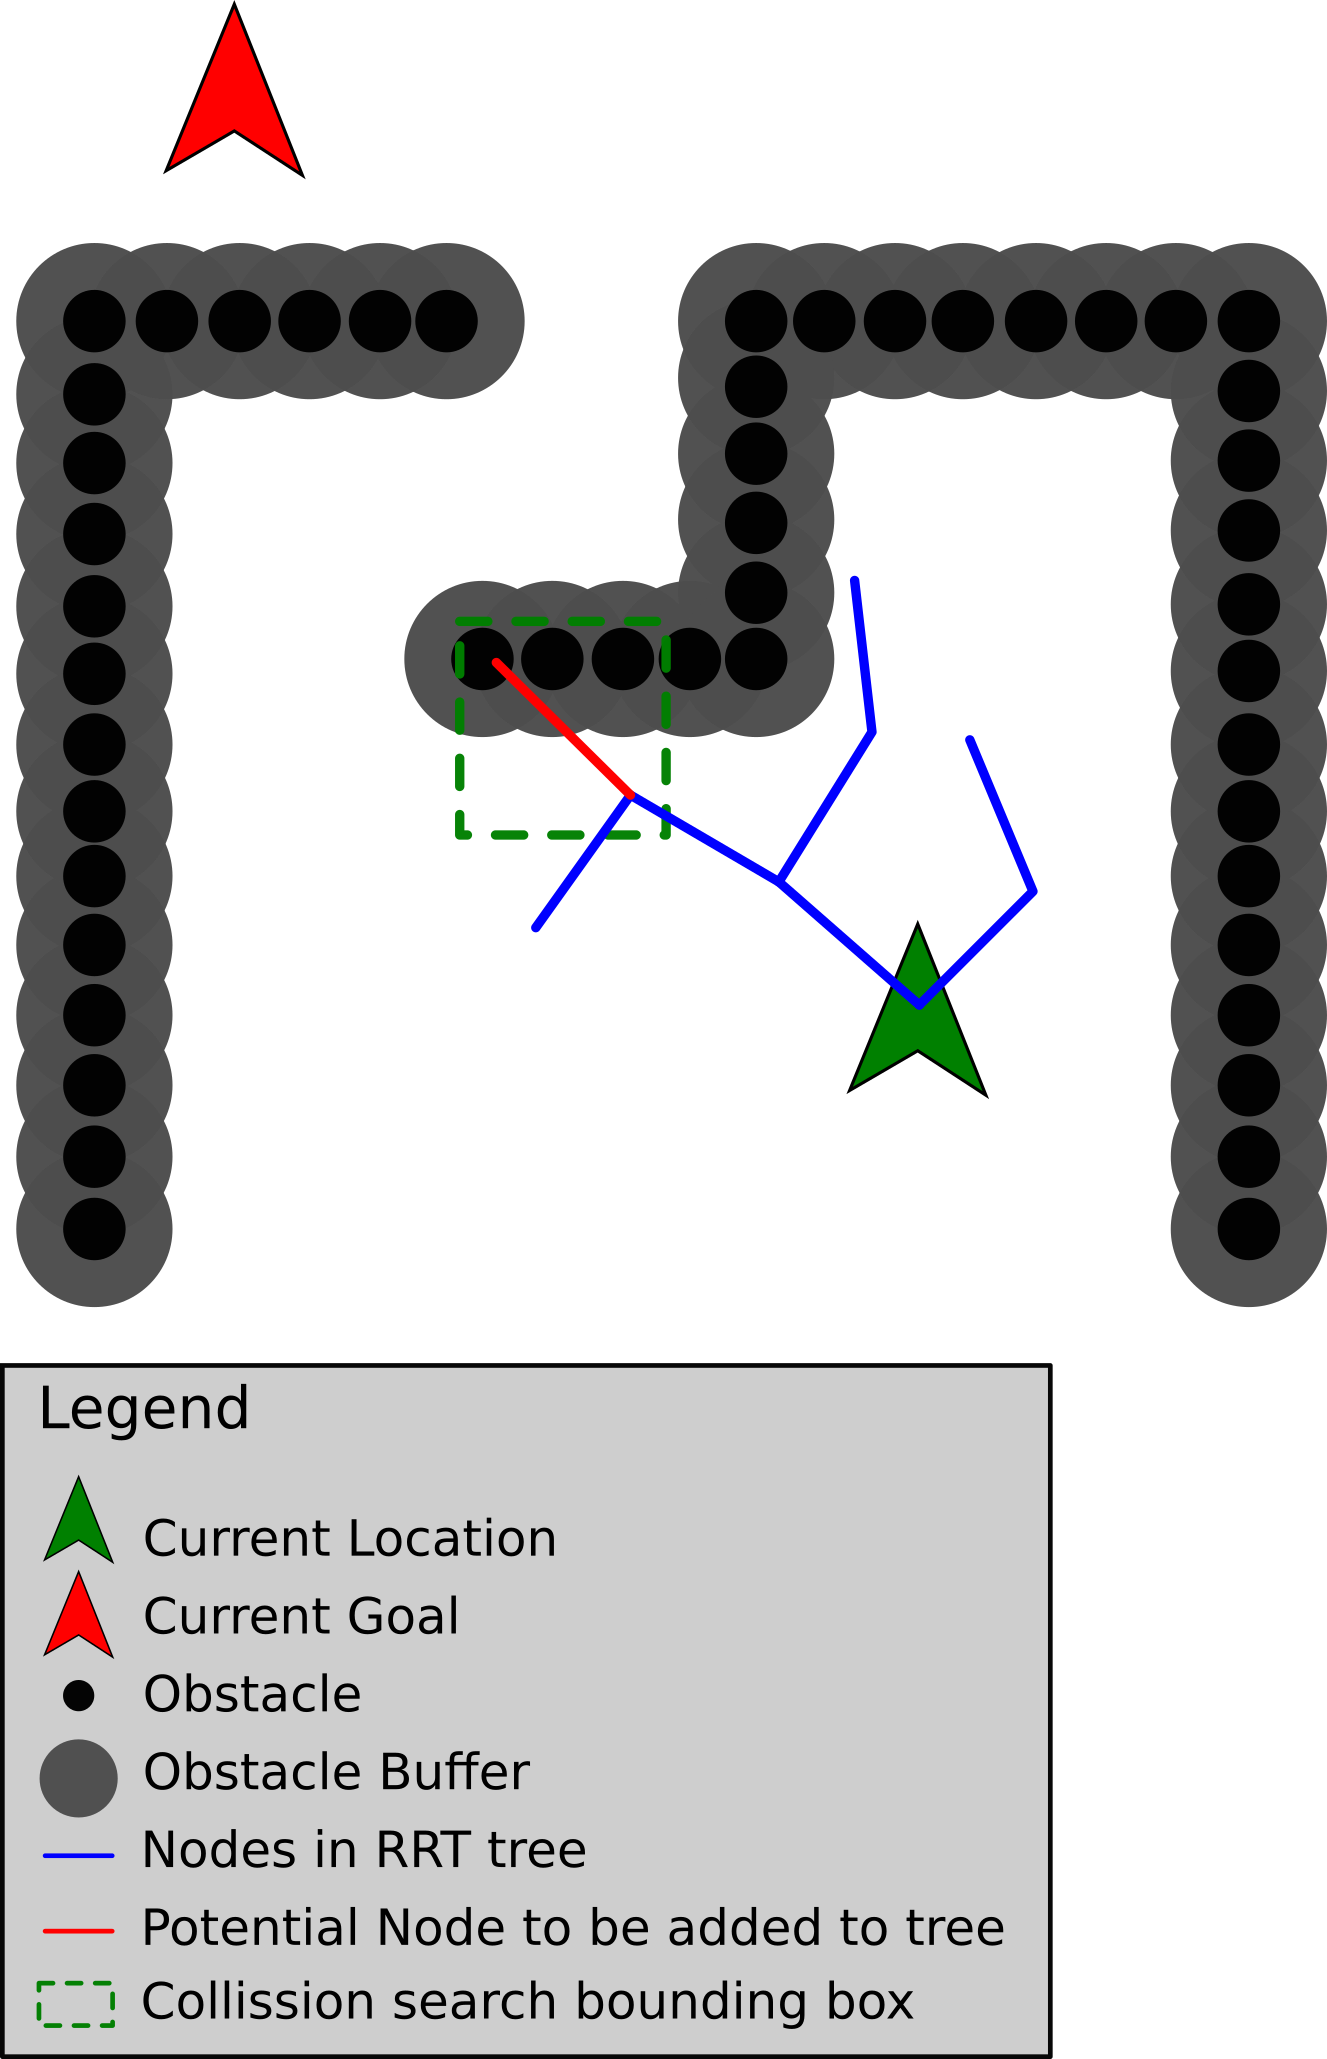
\includegraphics[width=0.8\linewidth]{rrt_sample}
\caption{Example of one step of collision check with the RRT planner.}
\label{fig:rrt_sample}
\end{figure}

As the RRT branches propagate, before each candidate node is added to the tree, an obstacle collision check is done only on the obstacles within range of the new node. The obstacles are determined to be in range according to the following algorithm.

\begin{algorithm}
  \caption{Obstacle Range Filter}
  \label{dyn_path_plan}
\begin{algorithmic}
  \REQUIRE $\mathit{candidate\_branch}$, $\mathit{obstacle\_list}$, $r_{\mathit{buf}}$
  \FORALL{$\mathit{obstacles}$ in $\mathit{obstacle\_list}$}
    \IF{$x_{\mathit{obs}} + r_{\mathit{buf}} \leq \min{(x_1, x_2)}$}
      \STATE continue
    \ELSIF{$x_{\mathit{obs}} - r_{\mathit{buf}} \geq \max{(x_1, x_2)}$}
      \STATE continue
    \ELSIF{$y_{\mathit{obs}} + r_{\mathit{buf}} \leq \min{(y_1, y_2)}$}
      \STATE continue
    \ELSIF{$y_{\mathit{obs}} - r_{\mathit{buf}} \geq \max{(y_1, y_2)}$}
      \STATE continue
    \ELSE
      \STATE $\mathit{filtered\_obstacles} \gets \mathit{obstacle}$
    \ENDIF
  \ENDFOR
  \RETURN $\mathit{filtered\_obstacles}$
\end{algorithmic}
\end{algorithm}

 $(x_1,y_1)$ and $(x_2,y_2)$ are the endpoints of the candidate branch, $(x_{\mathit{obs}},y_{\mathit{obs}})$ is the location of the obstacle being checked, and $r_{\mathit{buf}}$ is the buffer radius for each obstacle. The green bounding box in Fig. \ref{fig:rrt_sample} shows which obstacles would be included in the filtered obstacles after this check. The perpendicular distance between the candidate line (shown in red) and the filtered obstacles is checked with the following equations.

\begin{align}
  d &= \dfrac{|\Delta y*x_{\mathit{obs}} -
      \Delta x*y_{\mathit{obs}} + \Delta s|}
      {\sqrt{\Delta y^2 + \Delta x^2}}\\
  \nonumber \text{with}\\
  \Delta x &= x_2 - x_1\\
  \Delta y &= y_2 - y_1\\
  \Delta s &= x_2*y_1 -x_1*y_2
\end{align}

 If the distance $d$ is less than the buffer radius, a collision is detected and the candidate is rejected. By only checking for collisions with obstacles within the bounding box, nearly all obstacles are ignored for each step of propagation. This significantly improves performance of the RRT planner and allows it to plan in real time and dynamically update the path whenever needed. The collision detection for path smoothing and path checking works the same way, with $(x_1,y_1)$ and $(x_2,y_2)$ being the endpoints of each path segment.

% \subsection{Path Planning Algorithm}
% The path planning breaks down to four separate functions. The RRT planner, collision checker, path smoother, and path checker. Each time the obstacles are updated, the path checker is run to see if the current path is still valid. If invalid, the RRT planner is run from the current location then the path is smoothed following the
%
%
% \begin{algorithm}
%   \caption{Dynamic Path Planner}
%   \label{dyn_path_plan}
% \begin{algorithmic}
%     \IF{some condition is true}
%         \STATE do some processing
%     \ELSIF{some other condition is true}
%         \STATE do some different processing
%     \ELSE
%         \STATE do the default actions
%     \ENDIF
% \end{algorithmic}
% \end{algorithm}
%
%
% \todo{include algorithm section to explain what the planner is doing? or just more explanation? or is this good enough?}

%%%%%%%%%%%%%%%%%%%%%%%%%%%%%%%%%%%%%%%%%%%%%%%%%%%%%%%%%%%%%%%%%%%%%%%%%%%%%%%%
\section{Map Merging}\label{merge}

The map merging process we use is able to generate a combined map from multiple agents on a base station computer in near real-time while the UAVs are still mapping the environment.

Fig. \ref{fig:map_merge} shows the network diagram of the process of merging the maps. To merge the maps in near real time, each time a new keyframe is initialized, the data from the images consisting of the color and depth information from the keyframe, and the feature descriptions extracted from the color image are stored in a database referred to as RGB-D Cache which is hosted on the base station computer. A 3D color and depth (XYZRGB) pointcloud is generated using the color and depth information from the RGB-D camera and the features are generated from either SIFT/SURF or ORB using OpenCV.

\begin{figure*}
\centering
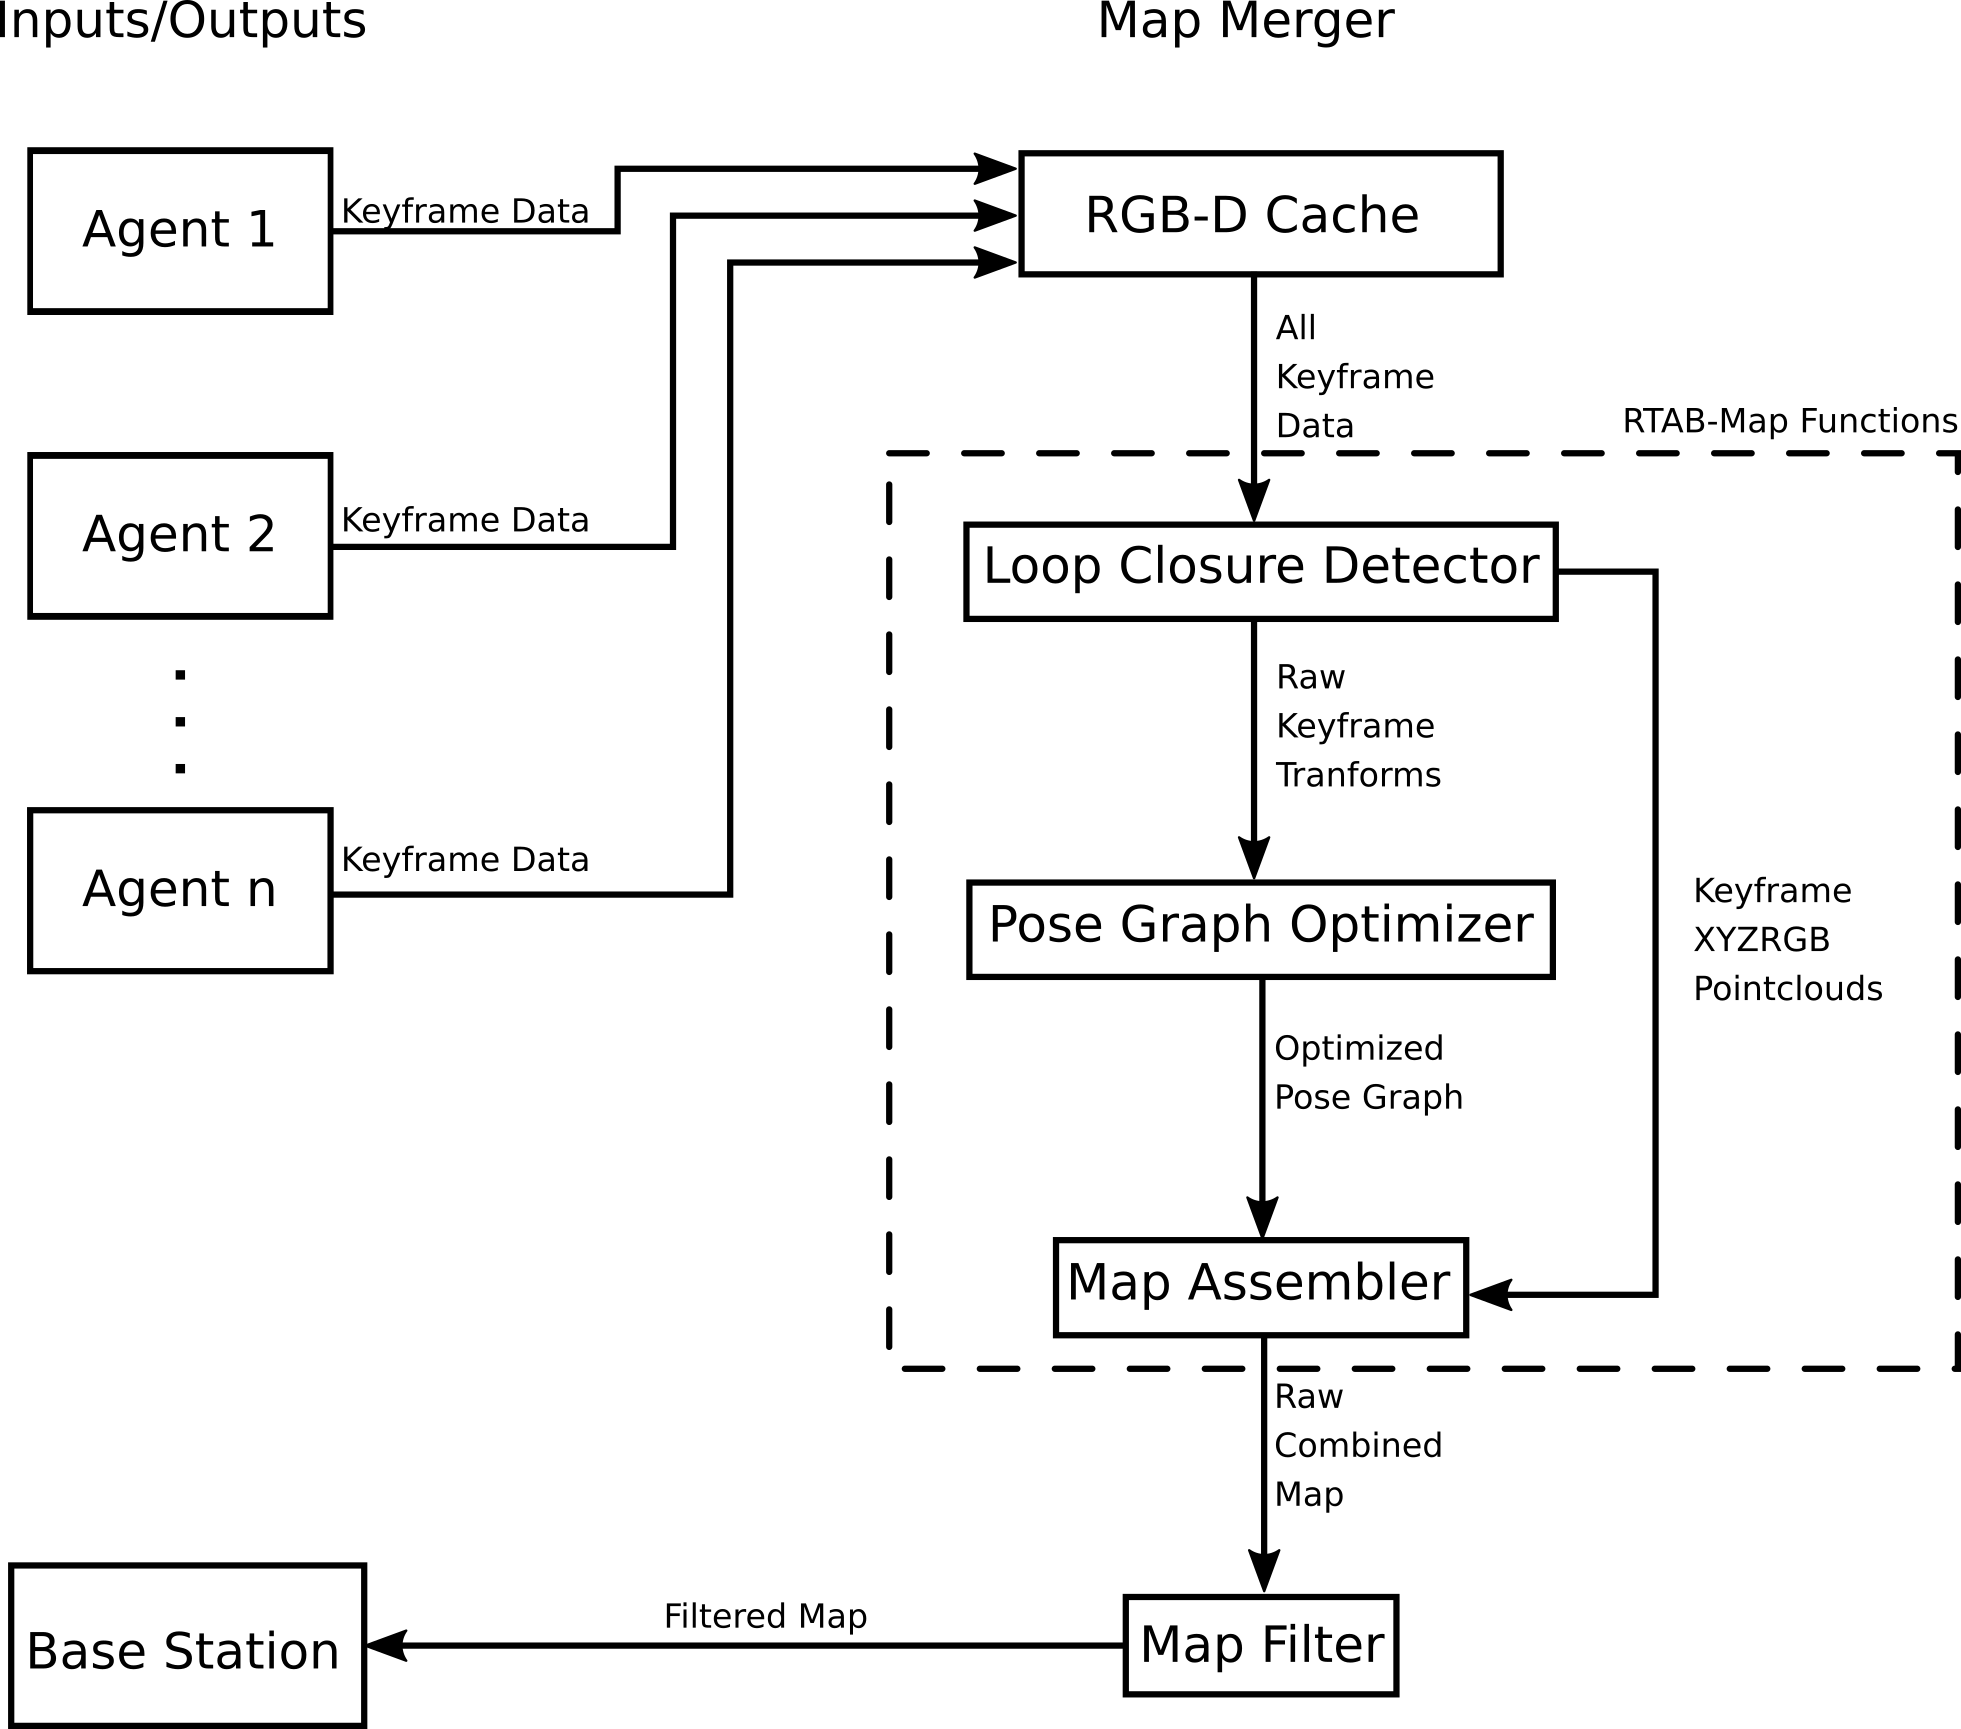
\includegraphics[width=0.7\linewidth]{map_merger_network}
\caption{The network diagram for the multi-agent map merging node proposed in this section.}
\label{fig:map_merge}
\end{figure*}

Once the database has been initialized, the maps are periodically merged using functions from an instance of RTAB-Map running on the base station computer similarly to how individual maps are generated for each UAV \cite{Labbe2011}\cite{Labbe2013}\cite{Labbe2019}. The first step is to search for loop closures in the image features from each keyframe using a bag-of-words approach. Rather than only look for loop closures from the keyframes of a single agent, this process looks for loop closures from all keyframes from all agents. Each time a new loop closure is found, a new edge is added to combined map graph with an estimated transformation between keyframes. After finding all loop closures with the current dataset, the graph is optimized using the pose graph optimizer built into RTAB-Map, the optimized pose graph is then sent to the map assembler along with the XYZRGB pointcloud from each keyframe where the pointclouds are combined according to the optimized graph edges. This generates a single map with all keyframes that can be connected into a single graph. This map is then processed to remove some noise and filter out the ceiling to make the map more understandable to the operator.

Since the base station computer is merging the maps it is able to run in real time. The larger the grow, however, the longer it takes to re-optimize the the combined map. This causes the updated map to lag behind real time.
%%%%%%%%%%%%%%%%%%%%%%%%%%%%%%%%%%%%%%%%%%%%%%%%%%%%%%%%%%%%%%%%%%%%%%%%%%%%%%%%
\section{Results and Discussion}\label{results}

\subsection{Simulation}

We were able to successfully autonomously navigate and map a simulation environment in ROS Gazebo \cite{Gazebo} with multiple agents and combine the maps. The simulation environment was designed to be as close to the real world and hardware as possible. We used a software in the loop (SIL) version of ROSflight \cite{Jackson2016a}, an open source autopilot library built with ROS, to mimic the flight controller. We did not use any ground truth information in the simulation, all measurements were from simulated sensors with noise characteristics similar to hardware. Fig. \ref{fig:sim_setup} shows the simulation setup used to map the environment.

\begin{figure}
\centering
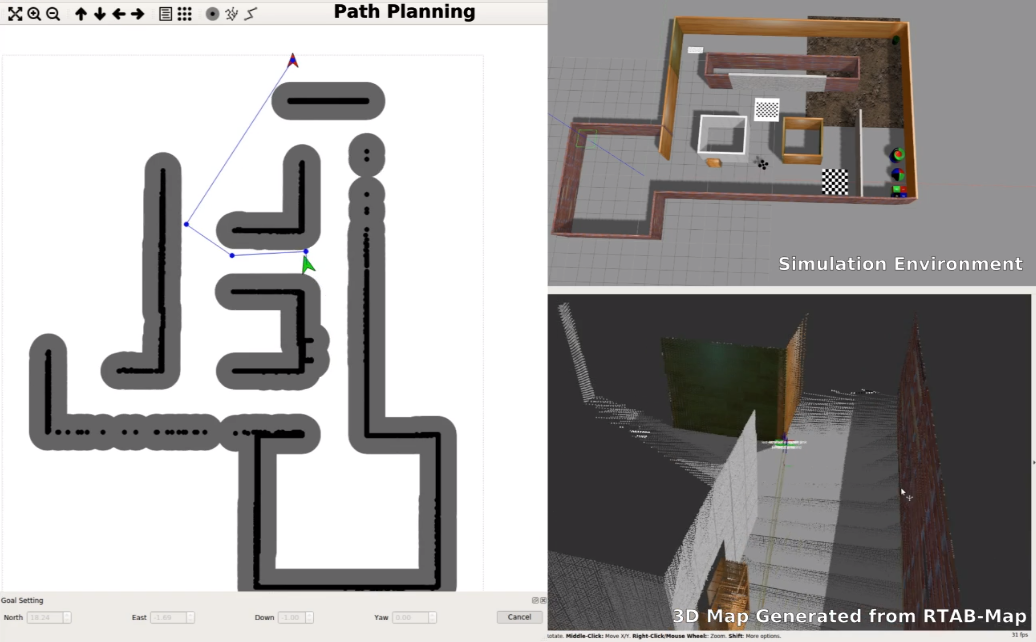
\includegraphics[width=1.0\linewidth]{sim_setup}
\caption{Setup used for the simulation results. The reactive planner is shown on the left, the simulation world is shown on the top right, and the current map is shown on the bottom right}
\label{fig:sim_setup}
\end{figure}

Fig. \ref{fig:sim_map} shows the results from mapping the simulated environment with two agents and combining the maps. Neither agent saw everything in the combined map, but the maps were successfully merged together into a single map with all features from each individual map.

\begin{figure}
\centering
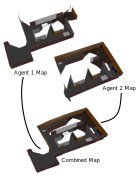
\includegraphics[width=1.0\linewidth]{sim_map}
\caption{Map generated from combined maps in the simulated environment.}
\label{fig:sim_map}
\end{figure}

Flying in simulation helped prove out the reactive planner and obstacle avoidance. It was also helpful to debug and sort out the plumbing of the relative navigation framework and control schemes. The area where the simulation falls short, is with the computer vision applications such as visual odometry and loop closure detection. Gazebo is excellent at simulating realistic physics and dynamics, but the environments are significantly less detailed than the real world. This made designing a simulation world more difficult. If there is too little detail added to the world, the visual odometry algorithms often fail or perform poorly. If too much repetitive detail is used, RTAB-Map finds too many false loop closures and the mapping fails. The simulated world developed and used to obtain results as shown in Figs. \ref{fig:sim_setup} and \ref{fig:sim_map} is able to minimize these issues, but still failed to produce results on par with a real world test. There are only a few locations where there is enough unique detail that loop closures will be detected, where nearly all locations in a real world environment have enough detail for loop closures. After proving the setup in high-fidelity simulation, we moved to hardware to get results especially with the computer vision aspects of the research.

\subsection{Hardware}

We were able to successfully combine maps generated from multiple UAVs in near real-time with manual flight. Fig \ref{fig:lab_map} shows an example of a map built in a cluttered environment with large amounts of glass. Although noisy, it is evident that the map merging works in hardware and generates a usable map of the environment. This map was generated from from pushing two agents on carts rather than flying them for safety concerns. Fig \ref{fig:wilk3_map} shows an example of a map built from a more structured hallway environment with little glass. The map generated here is more structured than that of the cluttered environment. \todo{this map was built from manually flying the UAVs}. We were unable to tune the RMEKF sufficiently to fly autonomously in an uncontrolled environment for these results, but we were able to prove that with a sufficiently tuned estimator, the planning, control, and obstacle avoidance will work using the simulated world.

\begin{figure*}
\centering
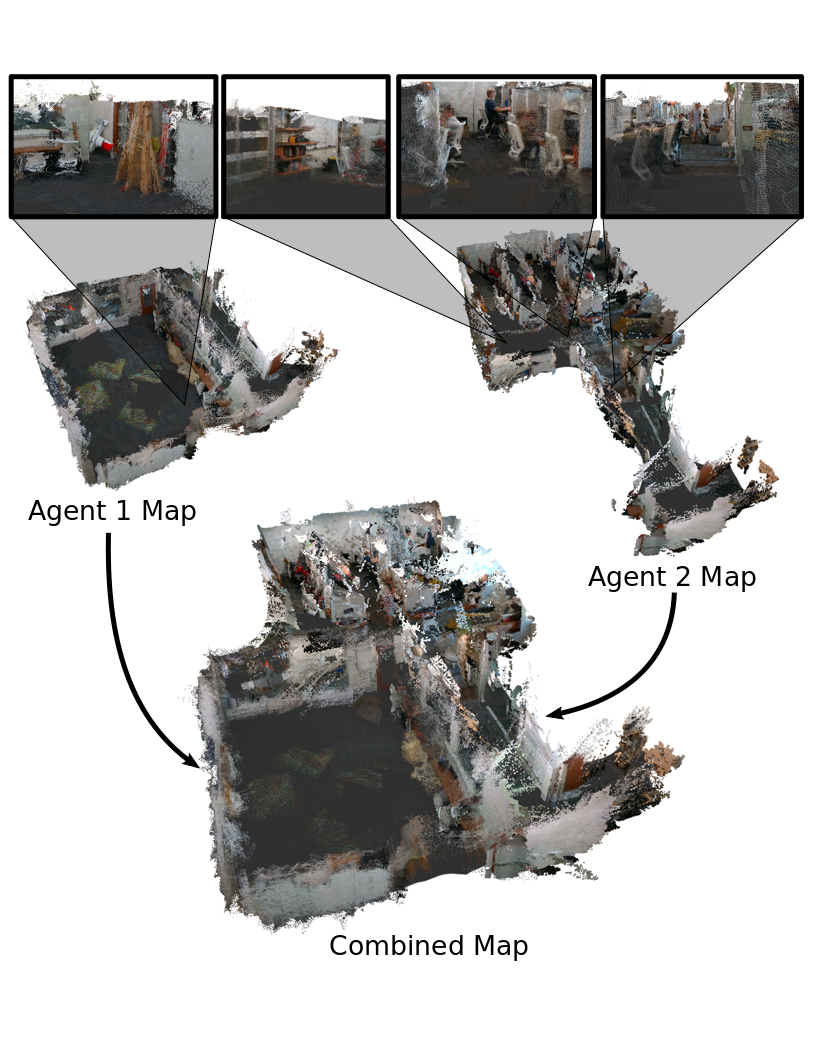
\includegraphics[width=0.9\linewidth]{lab_map.png}
\caption{Example of hardware results of merging maps from two agents into a single map in a cluttered environment. Above the individual agent maps are examples of the detail in the pointclouds when zooming in.}
\label{fig:lab_map}
\end{figure*}

\begin{figure*}
\centering
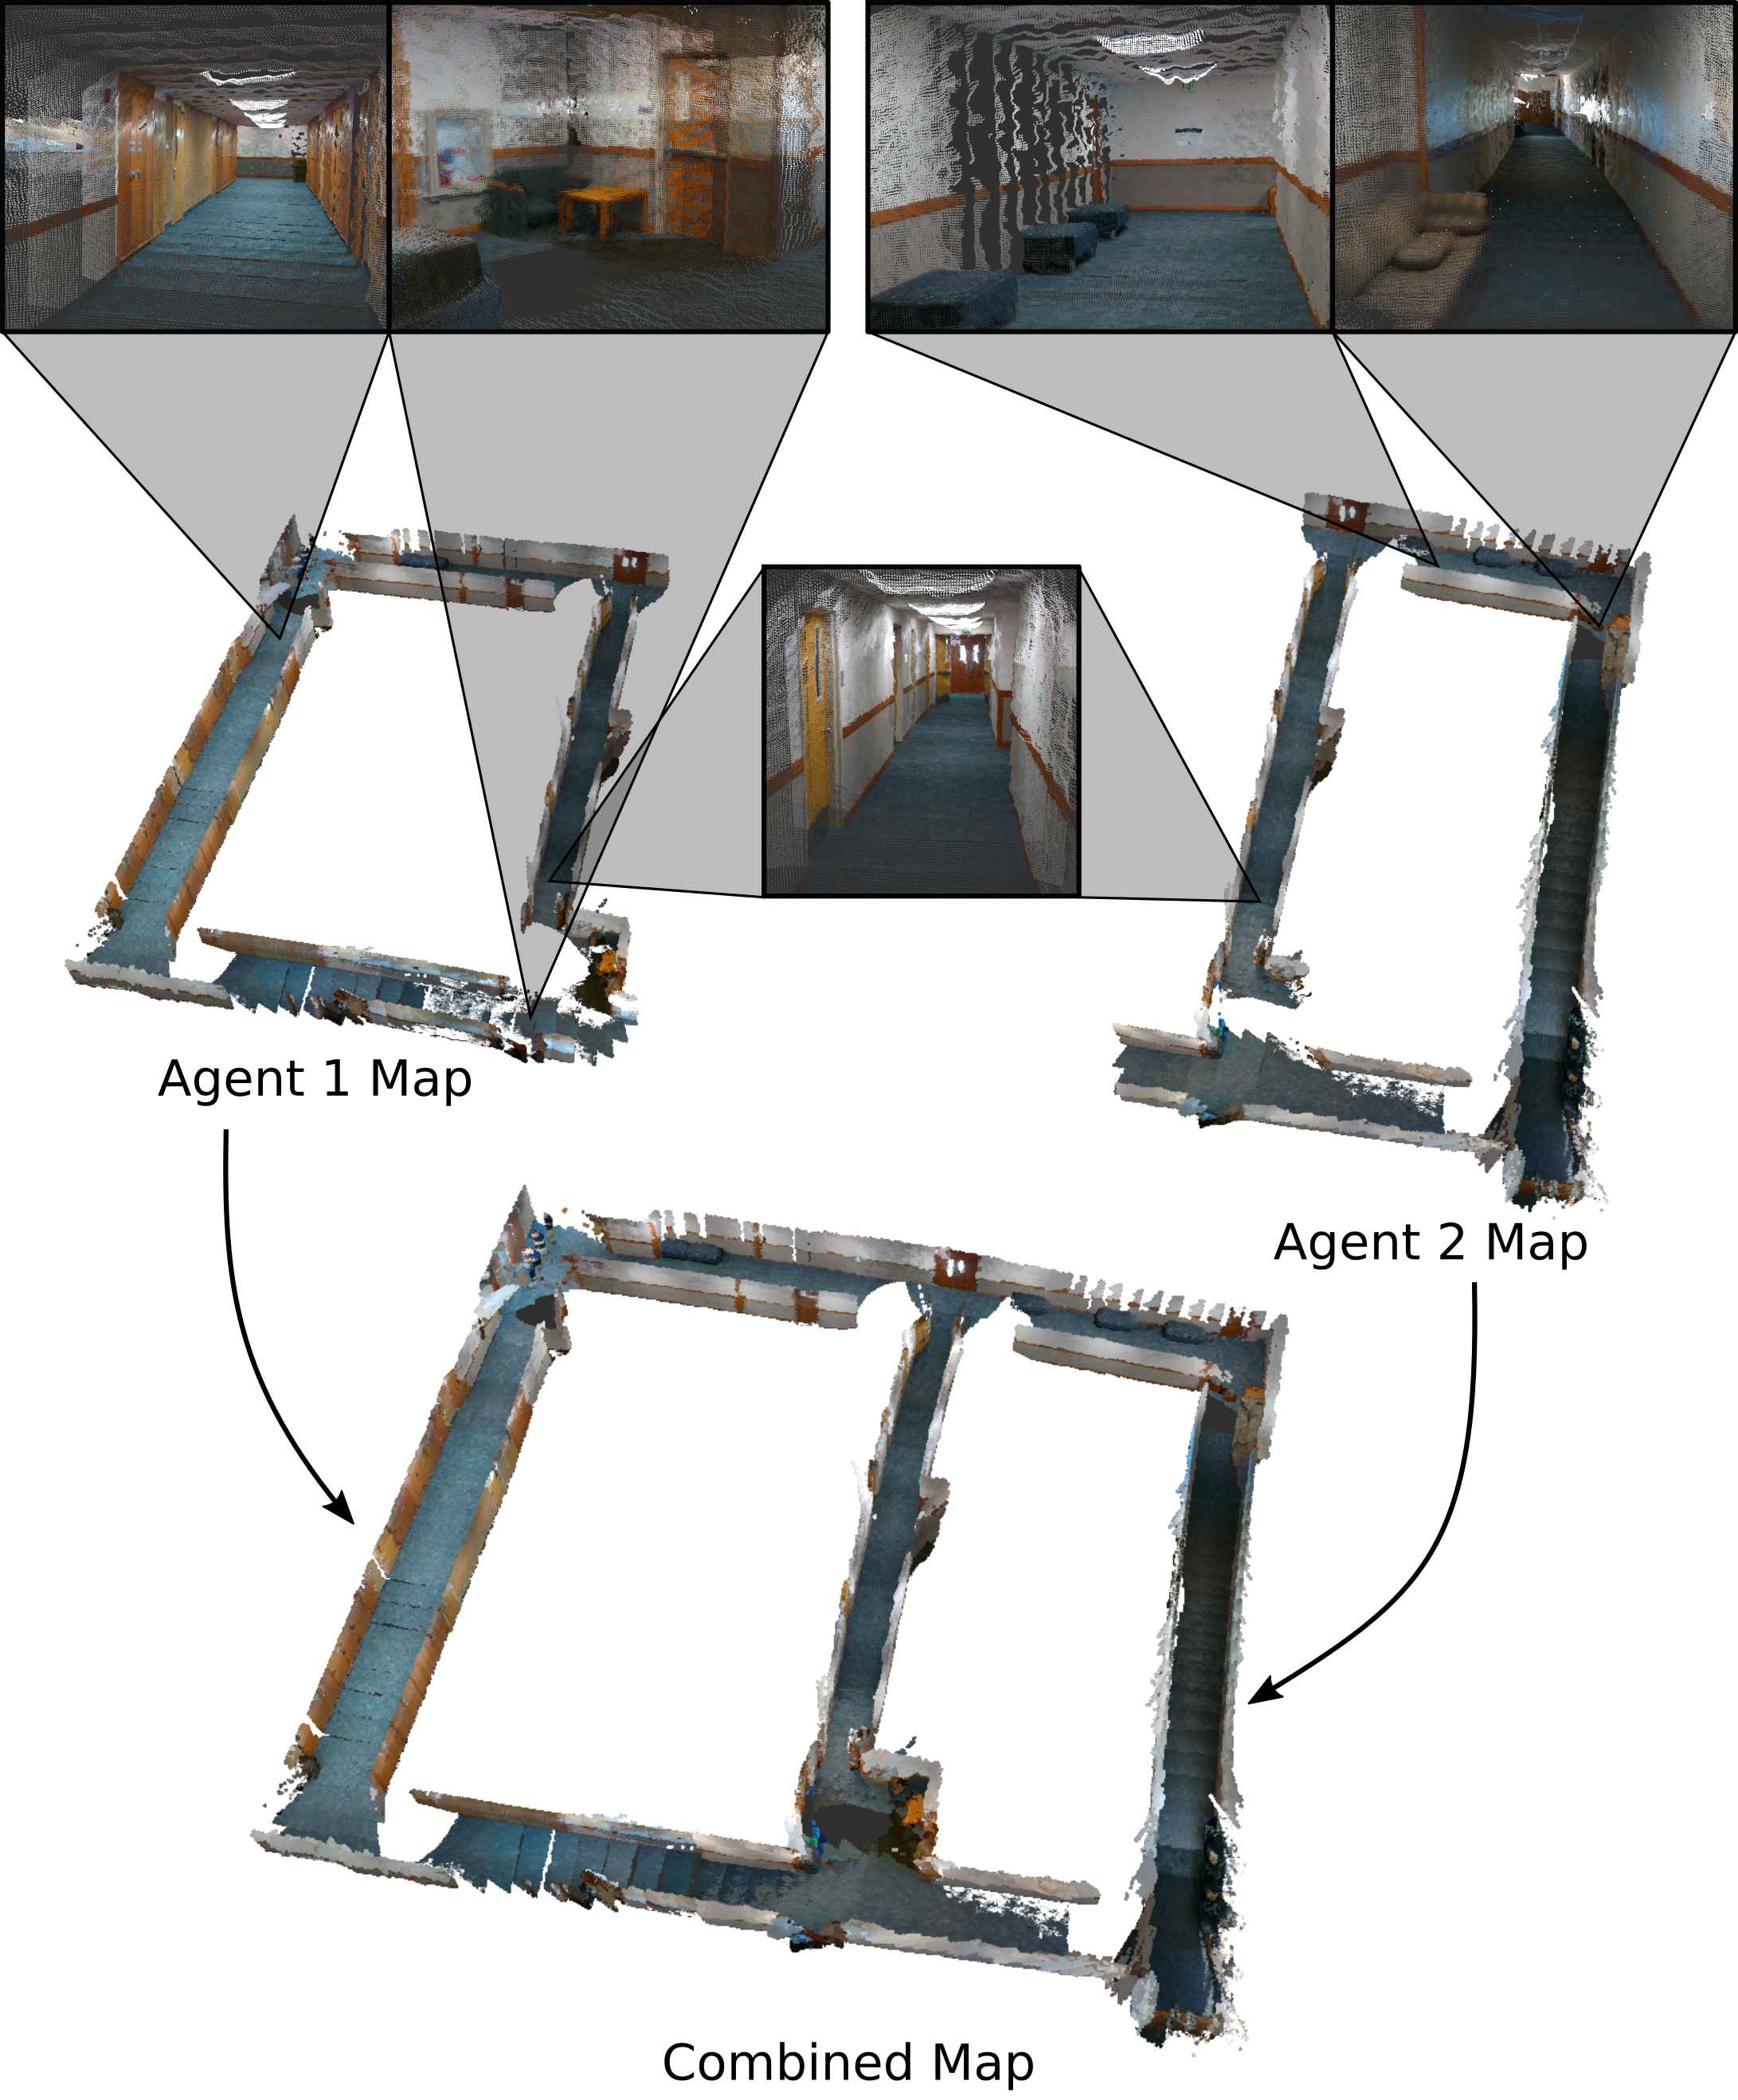
\includegraphics[width=0.9\linewidth]{wilk3_map.png}
\caption{Example of hardware results of merging maps from two agents into a single map in a simpler hallway environment. Above the individual agent maps are examples of the detail in the pointclouds when zooming in.}
\label{fig:wilk3_map}
\end{figure*}
%%%%%%%%%%%%%%%%%%%%%%%%%%%%%%%%%%%%%%%%%%%%%%%%%%%%%%%%%%%%%%%%%%%%%%%%%%%%%%%%
\section{Conclusions}\label{conclusions}

Using UAVs to generate dense 3D maps of GPS-Denied environments requires a careful choice of planning, estimation and mapping techniques to be successful. Using the combination of a reactive path planner and a CEPA obstacle avoidance velocity filter allows for navigation and exploration through complex GPS-Denied environments. Estimating relative and global states separately allows for the necessary decoupling of position and attitude controllers to fly autonomously without the use of GPS. Using multiple UAVs to collaboratively map an area improves mapping efficiency and when handled correctly, still allows the map building to occur in near real-time. Future work includes streamlining the map merging process to allow for full real-time map generation, improving the performance of the relative estimator to allow full autonomous flight in hardware, and connecting the UAVs to a high-level coverage path planner to allow for autonomous flight without human guidance.

%%%%%%%%%%%%%%%%%%%%%%%%%%%%%%%%%%%%%%%%%%%%%%%%%%%%%%%%%%%%%%%%%%%%%%%%%%%%%%%%

\bibliographystyle{IEEEtran} % We choose the "plain" reference style
\bibliography{mapping_paper_2019}

\end{document}
